\documentclass[11pt]{article}

\usepackage[margin=1in]{geometry}
\usepackage{amsmath, amssymb}
\usepackage{booktabs}
\usepackage{enumitem}
\usepackage{hyperref}
\usepackage{setspace}
\usepackage{graphicx}
\usepackage{xcolor}
\usepackage{array}

\setstretch{1.1}
\hypersetup{colorlinks=true, linkcolor=blue, urlcolor=blue, citecolor=blue}

\title{\textbf{Persona Carryover Under Matched Controls: History Compression, Strong Updates, and Warmup Reinforcement in Gemini-2.5-Flash-Lite}}
\author{Group ID: [To Fill] \\ [Member Names]}
\date{}

\begin{document}
\maketitle
\vspace{-1em}

\begin{abstract}
We study whether a language model still carries residual influence from a previously assigned persona after the system prompt is switched to a new target persona.
Our pipeline uses matched controls, premise libraries, and three task families: MBTI multiple-choice questions, open-ended Machine Mindset prompts, and IFEval instruction-following items.
RQ1 compares raw conversation history against compressed summaries and shows that summary-based retention is substantially more effective for clean persona switching.
RQ2 introduces a stronger final switch prompt and tests whether stronger late instructions can repair failed switches.
RQ3 strengthens the pre-switch warmup to test whether deeper early conditioning amplifies carryover.
Across the completed experiments, the strongest and most stable signal appears in the MBTI task: summary retention reaches the target persona much more often than history retention, stronger final instructions provide selective but incomplete repair, and reinforced warmup increases carryover even after stable-control filtering.
Premise filtering is critical: four MBTI types are unstable in the default premise library, so downstream RQ1 analyses are restricted to the resulting 132 directed pairs, and downstream RQ2 uses only personas that self-match in both default and strong premise libraries.
The overall picture is that persona carryover is real, it is highly sensitive to how prior context is retained, and prompt strengthening is a weaker control lever than reducing the amount of raw pre-switch context that directly survives into the final run.
\end{abstract}

\section{Introduction}

Large language models are often deployed under hidden contextual variation: system personas, prior conversation traces, and intermediate summaries may differ even when the final user instruction is identical.
This raises a reliability question: if a model is first conditioned to behave like persona $A$ and then explicitly switched to persona $B$, does it actually become $B$, or does part of $A$ leak into the final behavior?
This question matters for prompt-based alignment, multi-stage agents, and evaluation protocols that implicitly assume the latest system instruction dominates earlier context.

Our project falls under the course theme of behavioral variability under implicit conditions.
We focus on persona switching because it offers a controlled setting in which the target state is interpretable and testable.
Instead of asking whether personas change outputs in general, we ask whether earlier personas persist after an explicit switch, how that persistence depends on the representation of prior context, and whether stronger post-switch or pre-switch interventions alter the effect.

\textbf{Contribution summary.}
\begin{itemize}[leftmargin=*]
    \item We build a matched-control evaluation pipeline for persona carryover using three task families and pairwise MBTI persona switches.
    \item We show that premise validation is not optional: four MBTI types fail default self-match, and strong prompts repair only part of this instability.
    \item We provide a logically closed RQ1 analysis with pair filtering, forward-reverse symmetry checks, distance stratification, and dimension-level carryover patterns.
    \item We show that stronger final instructions help selectively rather than universally, while stronger pre-switch warmup increases carryover in both retention tracks once unstable matched controls are excluded.
    \item We identify matched-control drift as a systematic failure mode, especially for target ENTJ, indicating that downstream failures cannot be attributed solely to failed switch conditions.
\end{itemize}

\section{Related Work}

Our work is closest to recent studies on behavioral variability and persona effects in LLMs.
\cite{chen2023behavior} shows that model behavior can drift across time even under seemingly stable settings.
\cite{persona2024quantifying} quantifies the effect of personas in simulation settings, but does not isolate post-switch residual influence with matched controls.
\cite{greedy2024nondeterminism} and \cite{deterministic2025nondeterminism} emphasize that repeated LLM evaluation should not assume perfect determinism even under low-temperature settings.
\cite{helpful2024personas} argues that persona prompts do not reliably improve task performance, which aligns with our finding that a stronger final persona prompt is helpful only in specific retention settings.
\cite{control2025illusion} further motivates our design by showing that instruction hierarchies can fail when earlier context continues to influence model behavior.

Our study differs from prior work in three ways.
First, we focus on \emph{carryover after a switch}, not just the direct effect of adding a persona.
Second, we use matched controls of the form $B \rightarrow B$, so the final target persona is held fixed and only the earlier context differs.
Third, we decompose the effect by retention mechanism, pair direction, persona distance, and MBTI dimension, which lets us move beyond a single aggregate mean.

\section{Experimental Setup}

\subsection{Research Questions}

We study three linked questions.

\begin{itemize}[leftmargin=*]
    \item \textbf{RQ1:} Does a previously assigned persona $A$ still influence behavior after the final system prompt is switched to target persona $B$?
    \item \textbf{RQ2:} If the final switch prompt is made stronger, does switching become cleaner and more consistent with the matched $B \rightarrow B$ control?
    \item \textbf{RQ3:} If the pre-switch warmup is reinforced, does carryover become stronger and switching become harder?
\end{itemize}

Each question is operationalized in matched form.
RQ1 compares $A \rightarrow B$ against $B \rightarrow B$.
RQ2 compares the default switch conditions against strong-update counterparts such as \texttt{A\_summary\_to\_B\_strong}.
RQ3 compares the default switch conditions against reinforced warmup conditions such as \texttt{A3\_history\_to\_B}.

\subsection{Model, Tasks, and Data}

All completed experiments in this report use \texttt{gemini-2.5-flash-lite}.
We evaluate three task families so that persona carryover is measured both on direct personality probes and on downstream behavioral tasks.

\begin{center}
\small
\begin{tabular}{@{}p{0.24\linewidth} p{0.14\linewidth} p{0.54\linewidth}@{}}
\toprule
\textbf{Dataset} & \textbf{Size} & \textbf{Purpose} \\
\midrule
MBTI questions & 93 & Directly infer the final MBTI profile and target-persona reach after switching \\
Machine Mindset & 30 & Open-ended self-awareness prompts scored by a reference-bank semantic similarity pipeline \\
IFEval & 30 & Instruction-following tasks used to test whether persona carryover spills into constraint adherence \\
\bottomrule
\end{tabular}
\end{center}

The MBTI task is the most direct carryover probe, because its output can be aggregated into a final four-letter type.
Machine Mindset and IFEval provide complementary views: one semantic and one instruction-following.

\subsection{Condition Design}

We work with 16 MBTI personas.
For RQ1, every ordered pair $(A,B)$ with $A \neq B$ is a candidate directed switch pair, giving $16 \times 15 = 240$ directed pairs before filtering.
The switch pipeline contains three phases:
\begin{enumerate}[leftmargin=*]
    \item a warmup phase under persona $A$ or $B$,
    \item a retention step, either \texttt{history} or \texttt{summary},
    \item a final evaluation phase under target persona $B$.
\end{enumerate}

The two retention mechanisms are central to the design:
\begin{itemize}[leftmargin=*]
    \item \textbf{History:} the raw earlier dialogue is carried into the final run.
    \item \textbf{Summary:} the earlier dialogue is compressed into a summary before the final run.
\end{itemize}

This separation lets us test whether the model is sensitive to the \emph{content} of earlier conditioning or to the \emph{form} in which it is retained.

\subsection{Premise Libraries and Pair Filtering}

Before comparing switch conditions, we first ask whether a persona can even self-induce reliably under an \texttt{MBTI\_only} premise run.
This premise library serves as a validity screen.
If a target persona cannot reliably self-match in premise mode, then a later switch failure may reflect poor persona controllability rather than genuine carryover.

Table~\ref{tab:premise} summarizes the premise results.
Under the default premise library used for RQ1, only 12 of the 16 MBTI types self-match exactly.
The unstable personas are ESFP, ESTP, ISFP, and INTP.
Therefore, all downstream RQ1 analyses are restricted to the remaining $12 \times 11 = 132$ directed pairs.

RQ2 introduces a strong premise library.
It improves self-match from 12/16 to 14/16 by repairing ESTP and INTP, while ESFP and ISFP remain unstable.
However, to keep RQ1--RQ2 comparisons fair, we restrict downstream RQ2 analyses to the \emph{intersection} of personas that self-match in both libraries, which is still 12 personas.
This keeps the pair universe fixed rather than allowing the premise screen itself to change the population under comparison.

\begin{table}[t]
\centering
\small
\begin{tabular}{@{}lccc@{}}
\toprule
\textbf{Premise library} & \textbf{Exact self-match} & \textbf{Unstable types} & \textbf{Stable in both} \\
\midrule
RQ1 default premise & 12 / 16 & ESFP, ESTP, ISFP, INTP & -- \\
RQ2 strong premise & 14 / 16 & ESFP, ISFP & -- \\
Intersection used downstream & -- & -- & 12 / 16 \\
\bottomrule
\end{tabular}
\caption{Premise-library screening before downstream pair analysis.}
\label{tab:premise}
\end{table}

\subsection{Downstream Pair Selection for RQ2 and RQ3}

After filtering to the 132 eligible RQ1 pairs, we group each pair by whether the two RQ1 switch tracks succeed.
This yields 16 \texttt{Both Failed} pairs, 26 \texttt{Both Successful} pairs, and 90 \texttt{Mixed} pairs.

The \emph{full} downstream design is:
\begin{itemize}[leftmargin=*]
    \item \textbf{RQ2:} 60 pairs = 16 failed + 44 mixed.
    \item \textbf{RQ3:} 60 pairs = 26 successful + 34 mixed.
\end{itemize}

At the time of writing, the workspace contains a \emph{completed actual run pool} of 66 RQ2 pairs and 66 RQ3 pairs, because an initial 30+30 tranche was followed by a 36+36 supplement.
This executed pool is larger than the original 60+60 downstream design, so the final aggregation in this report is based on the complete executed runs rather than on an incomplete reconstruction of the original 60-pair plan.

For rigor, we apply one additional filter before aggregation:
\begin{itemize}[leftmargin=*]
    \item \textbf{RQ2 stable-control filter:} keep only pair-track cells whose default and strong $B \rightarrow B$ MBTI controls both end at target persona $B$.
    \item \textbf{RQ3 stable-control filter:} keep only pair-track cells whose simple and reinforced $B \rightarrow B$ MBTI controls both end at target persona $B$.
\end{itemize}

This produces the final empirical coverage used below:
\begin{itemize}[leftmargin=*]
    \item \textbf{RQ2:} 66 executed pairs, filtered to 60 stable history pair-tracks and 60 stable summary pair-tracks.
    \item \textbf{RQ3:} 66 executed pairs, filtered to 57 stable history pair-tracks and 61 stable summary pair-tracks.
\end{itemize}

\section{Metrics and Statistical Protocol}

\subsection{Evaluation Metrics}

We evaluate switching at the \emph{pair-task-track} level.
The three most important metrics are:

\begin{itemize}[leftmargin=*]
    \item \textbf{Primary gap to matched control:} how far the switch condition is from the matched $B \rightarrow B$ control on the task's primary metric.
    \item \textbf{SCS (Switch-Control Similarity):} agreement between the switch output and the matched control.
    \item \textbf{RAI (Residual A Influence):} how much the output still aligns with persona $A$ relative to the target persona $B$.
\end{itemize}

For MBTI, we also compute whether the final aggregated type exactly matches the target persona $B$.
This produces the most interpretable switch-success signal.

\subsection{Statistical Protocol}

Rather than reporting a single pooled mean, we rely on paired and stratified summaries:
\begin{itemize}[leftmargin=*]
    \item track-wise comparisons between history and summary,
    \item forward-versus-reverse pair symmetry checks,
    \item persona-distance stratification by 1, 2, 3, or 4 changed MBTI dimensions,
    \item per-dimension carryover analysis for EI, SN, TF, and JP,
    \item pair-level shares improved (RQ2) and weakened (RQ3).
\end{itemize}

This is a deliberately effect-size-oriented analysis protocol.
Because each result is already aggregated at the pair level under matched controls, our focus is on directional consistency, subgroup patterns, and failure modes rather than on a single global significance test.

\section{Results}

\subsection{RQ1: Carryover Exists, and Summary Dominates History}

RQ1 is the most complete part of the study: all 240 directed pairs were run, and downstream interpretation is restricted to the 132 pairs whose source and target personas both pass the premise screen.

The clearest finding appears in the MBTI task.
Under history retention, the switch reaches the target persona only 21.25\% of the time.
Under summary retention, the target reach rate rises to 72.92\%.
The same direction appears in the control-based metrics: on MBTI, summary reduces the average gap to the matched control from 0.3146 to 0.0396, improves mean SCS from 0.6627 to 0.8909, and turns mean RAI from positive carryover ($+0.1478$) to negative residual influence ($-0.3152$).

Machine Mindset shows a weaker but consistent version of the same pattern: summary lowers the mean primary gap from 0.0422 to 0.0180 and shifts mean RAI from $+0.0131$ to $-0.0477$.
IFEval is more neutral: the two tracks have similar primary gaps, suggesting that persona carryover affects personality-sensitive behavior more strongly than pure instruction-following.

\begin{figure}[t]
\centering
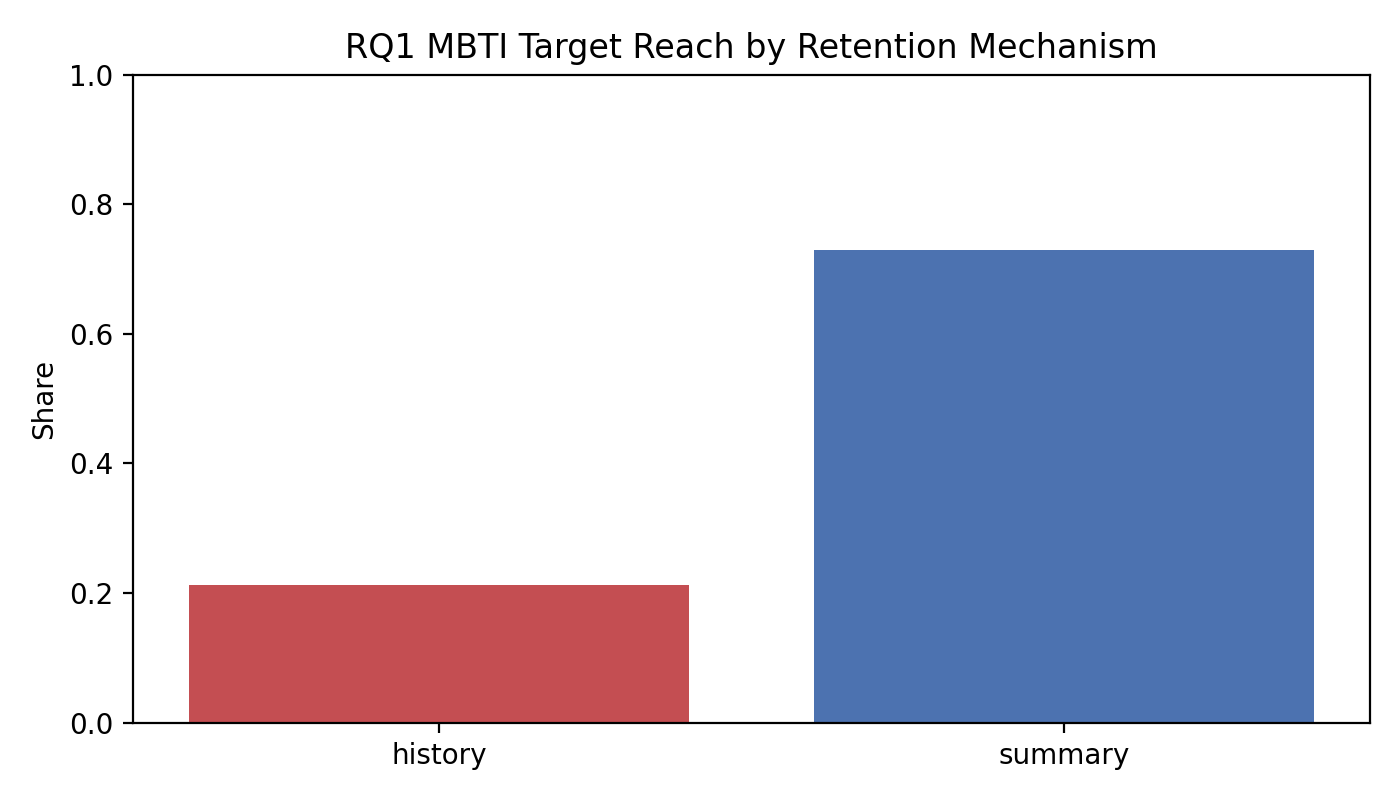
\includegraphics[width=0.62\linewidth]{final_report_assets/rq1_mbti_target_reach.png}
\caption{RQ1 MBTI target reach is dramatically higher under summary retention than raw history retention.}
\label{fig:rq1-target-reach}
\end{figure}

\subsection{Forward-Reverse Symmetry Is Only Partial}

If persona switching were fully symmetric, then for an unordered pair $\{A,B\}$ we would expect the outcomes for $A \rightarrow B$ and $B \rightarrow A$ to match.
They do not.

Among the 66 unordered pairs induced by the 12 stable personas, history is symmetric in only 44 cases (66.67\%), leaving 22 asymmetric cases.
Moreover, the symmetric history cases are overwhelmingly \emph{joint failures}: 42 unordered pairs fail in both directions, while only 2 succeed in both directions.
Summary is more symmetric overall (52 of 66, or 78.79\%), but the symmetric summary cases are overwhelmingly \emph{joint successes}: 51 unordered pairs succeed in both directions, while only 1 fails in both directions.

This shows that asymmetry is real, but it is layered on top of very different baselines.
History creates a regime where switching is hard in both directions; summary creates a regime where switching is usually easy in both directions.

\subsection{Persona Distance Matters, but Mainly for History}

We next stratify pairs by the number of MBTI dimensions that change between $A$ and $B$.
The history track degrades monotonically as distance grows:
\begin{itemize}[leftmargin=*]
    \item 1 dimension changed: 22.22\% target reach,
    \item 2 dimensions changed: 20.37\%,
    \item 3 dimensions changed: 17.65\%,
    \item 4 dimensions changed: 12.50\%.
\end{itemize}

Summary is much more robust.
For 1--3 changed dimensions, target reach stays near 0.88--0.91, and it falls only for the most extreme 4-dimension switches (62.5\%).
This implies that summary compression largely removes the burden of persona distance until the target persona is maximally far from the source persona.

\begin{figure}[t]
\centering
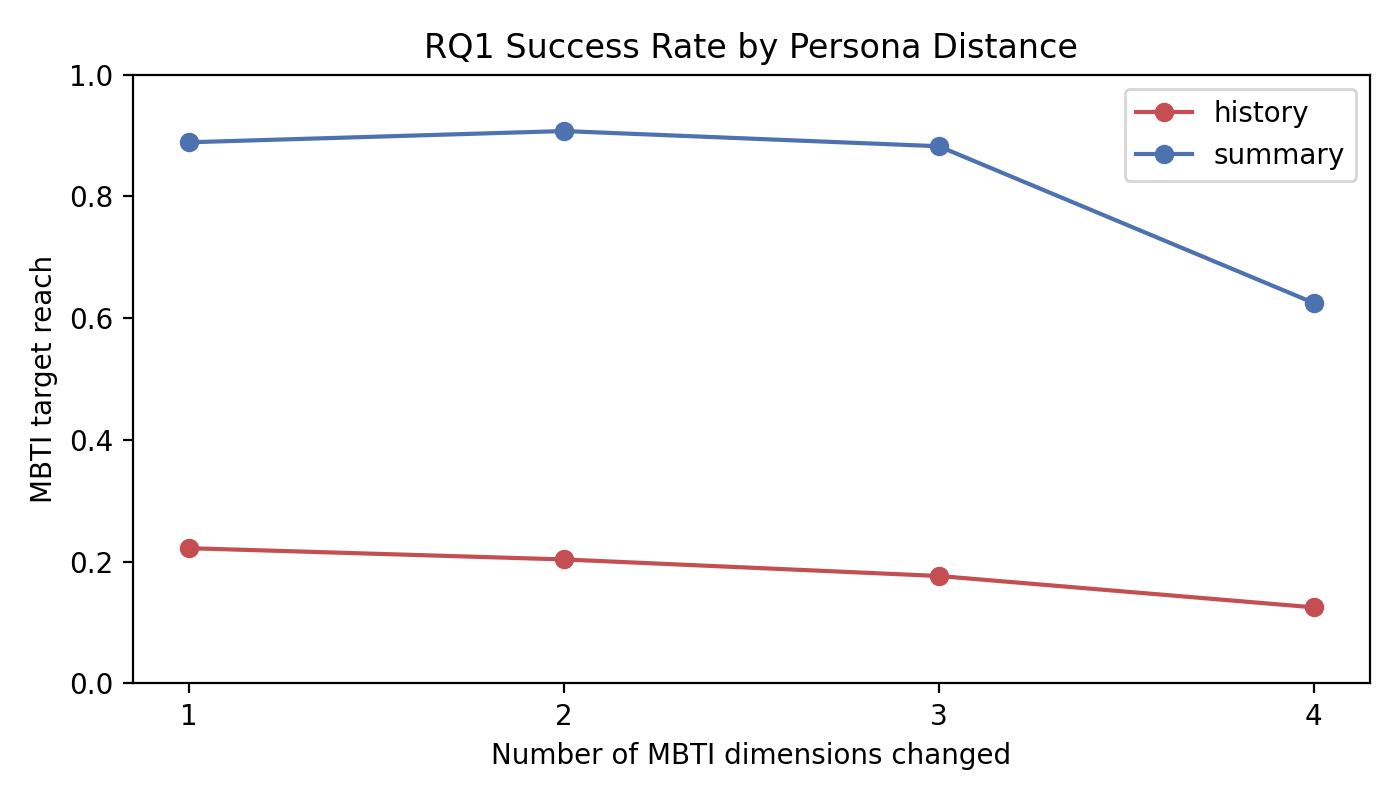
\includegraphics[width=0.7\linewidth]{final_report_assets/rq1_distance_success.png}
\caption{RQ1 MBTI target reach by the number of changed MBTI dimensions. Summary is robust through three changed dimensions; history declines steadily.}
\label{fig:rq1-distance}
\end{figure}

\subsection{Different MBTI Dimensions Show Different Carryover Patterns}

Dimension-level analysis reveals that carryover is not uniform across the four MBTI axes.
Under history retention, the final answer keeps persona $A$'s original letter most often on:
\begin{itemize}[leftmargin=*]
    \item TF: 77.78\%
    \item EI: 72.22\%
    \item SN: 70.00\%
    \item JP: 68.75\%
\end{itemize}

Under summary retention, the final answer adopts persona $B$'s target letter almost perfectly on EI and TF (both 100\%), remains very high on SN (91.43\%), and is weakest on JP (84.38\%).

Two conclusions follow.
First, TF and EI are the most ``sticky'' dimensions under raw history.
Second, JP remains the hardest dimension to rewrite even after compression, which suggests that not all persona traits are equally recoverable once earlier context is summarized.

\begin{figure}[t]
\centering
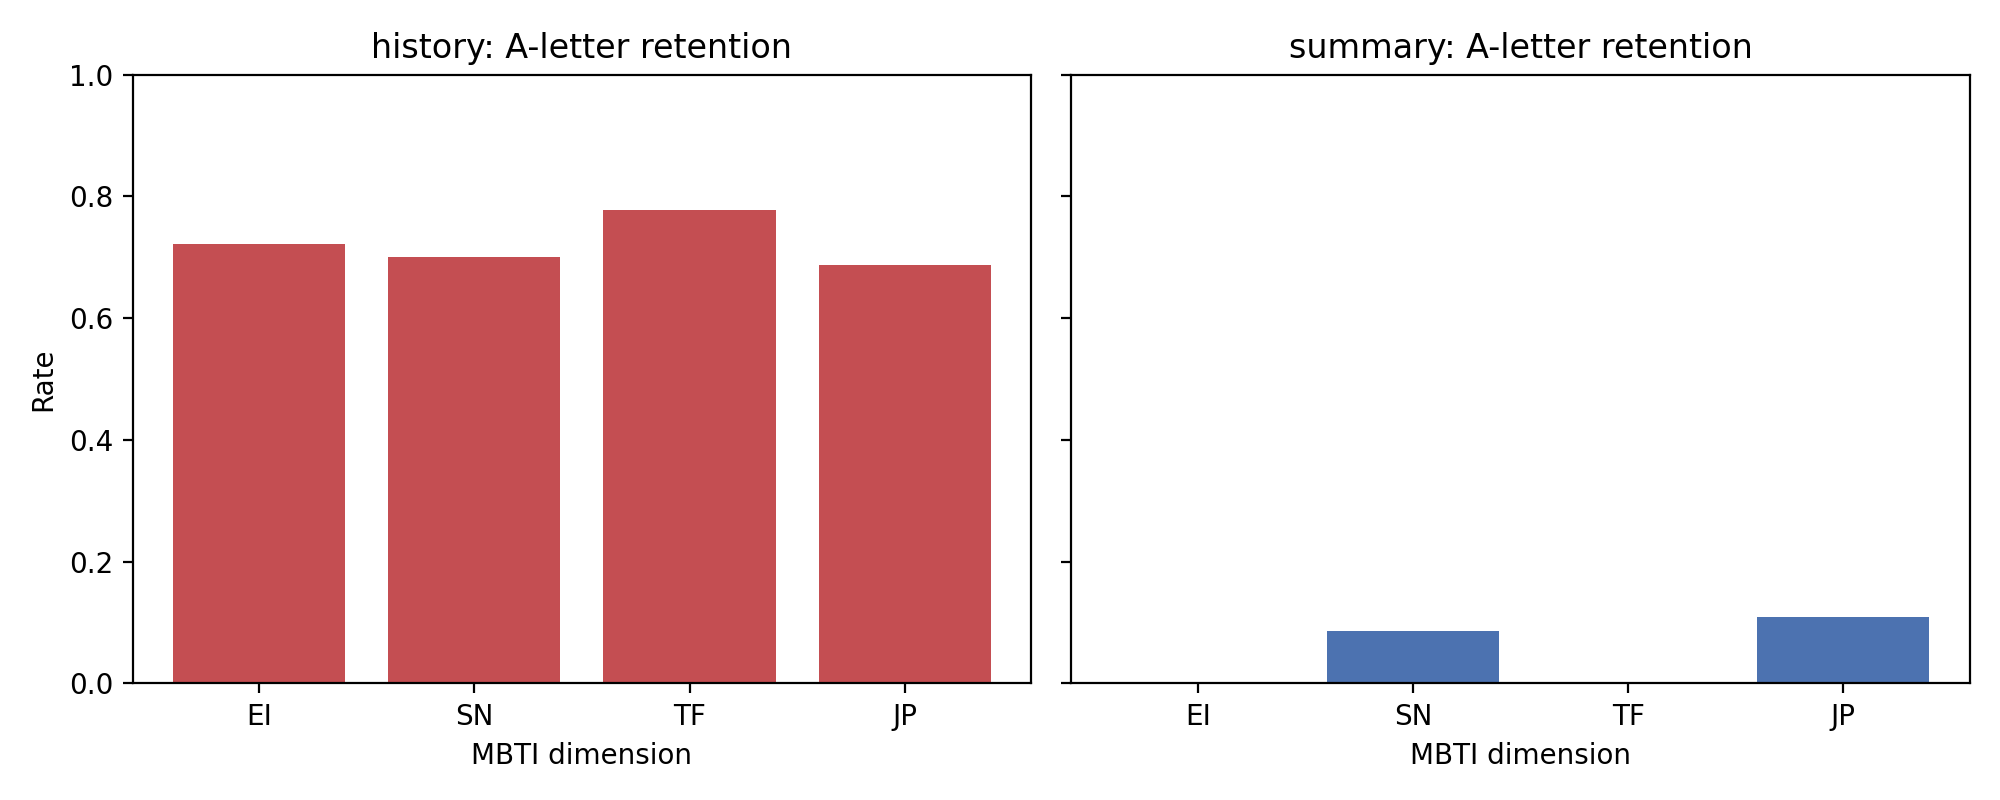
\includegraphics[width=0.84\linewidth]{final_report_assets/rq1_dimension_carryover.png}
\caption{Dimension-level RQ1 carryover. History retains persona-$A$ letters strongly, especially on TF and EI. Summary largely rewrites to persona-$B$, but JP remains less stable than EI and TF.}
\label{fig:rq1-dimension}
\end{figure}

\subsection{RQ2: Stronger Final Instructions Help, with the Clearest Gains in Summary MBTI}

RQ2 first changes the premise layer.
Strong prompting increases exact self-match from 12/16 to 14/16, repairing ESTP and INTP while leaving ESFP and ISFP unstable.
For fair comparison with RQ1, downstream RQ2 still uses the 12-person intersection and then applies the stable-control filter described above.

Among the 66 executed RQ2 pairs, six target-ENTJ pairs are removed because both the default and strong $B \rightarrow B$ controls drift to ESTJ.
After filtering, each retention track retains 60 stable pair-tracks.

The stable-control-filtered results show that stronger final instructions help, but not uniformly across tasks or retention modes.
On MBTI, improvement is observed in both tracks, with 30 of 60 stable history pairs (50.0\%) and 37 of 60 stable summary pairs (61.67\%) moving in the intended direction.
History exhibits the larger reduction in mean gap to the matched control ($-0.0708$), but summary remains the cleaner regime in absolute terms: mean SCS rises from 0.8688 to 0.9020 and residual A influence shifts further away from persona $A$ ($-0.0810$), indicating that the final behavior is more cleanly consolidated around the target persona.

The auxiliary tasks complicate this picture.
Machine Mindset benefits most under history, with 51 of 60 pairs improved (85.0\%), whereas summary is close to evenly split (48.33\% improved).
IFEval shows only modest gains, with 46.67\% improvement under history and 56.67\% under summary, and its lexical-similarity-based SCS decreases in both tracks.

Taken together, RQ2 supports a constrained conclusion.
Strengthening the final switch prompt is useful, but it does not erase the effect of earlier context.
Its most reliable benefit appears in MBTI summary switching, while other tasks show either weaker gains or mixed trade-offs.
This suggests that stronger late instructions can improve alignment to the target persona, but only within the limits imposed by the retained pre-switch context.

\subsection{RQ3: More Warmup Worsens Carryover, and Summary Is Not Immune}

RQ3 keeps the same logic but intensifies the pre-switch conditioning by using repeated warmup blocks before the final switch.
The executed run pool contains 66 pairs.
After stable-control filtering, 57 history pair-tracks and 61 summary pair-tracks remain.
The excluded cases are again structured rather than random: ENTJ targets drift to ESTJ in both tracks, while several ISTP targets drift to ISTJ only under reinforced history control.

On MBTI, reinforced warmup weakens switching in both tracks.
History is weakened in 32 of 57 stable pairs (56.14\%), and summary is weakened in 38 of 61 stable pairs (62.30\%).
The mean MBTI gap to matched control increases by $+0.0658$ under history and $+0.0410$ under summary, while mean SCS declines in both tracks.
Residual A influence also increases in both tracks, with a larger average rise under summary ($+0.0539$) than under history ($+0.0347$).

This is a substantive revision of the simpler picture suggested by the earlier tranche-level analysis.
Once unstable controls are excluded and the full completed run pool is used, stronger warmup is not merely a history-side vulnerability.
It can reintroduce measurable carryover even after prior context has been compressed into summary form.

The auxiliary tasks again show heterogeneous behavior.
Machine Mindset is weakened more often under summary (70.49\%) than under history (50.88\%), and IFEval is sharply asymmetric: only 22.81\% of stable history pairs are weakened, compared with 63.93\% of stable summary pairs.
The most defensible interpretation is therefore task-specific.
MBTI remains the cleanest direct probe of persona switching, while the downstream tasks also reflect stylistic persistence and semantic anchoring that are not fully captured by final-type matching alone.

\begin{figure}[t]
\centering
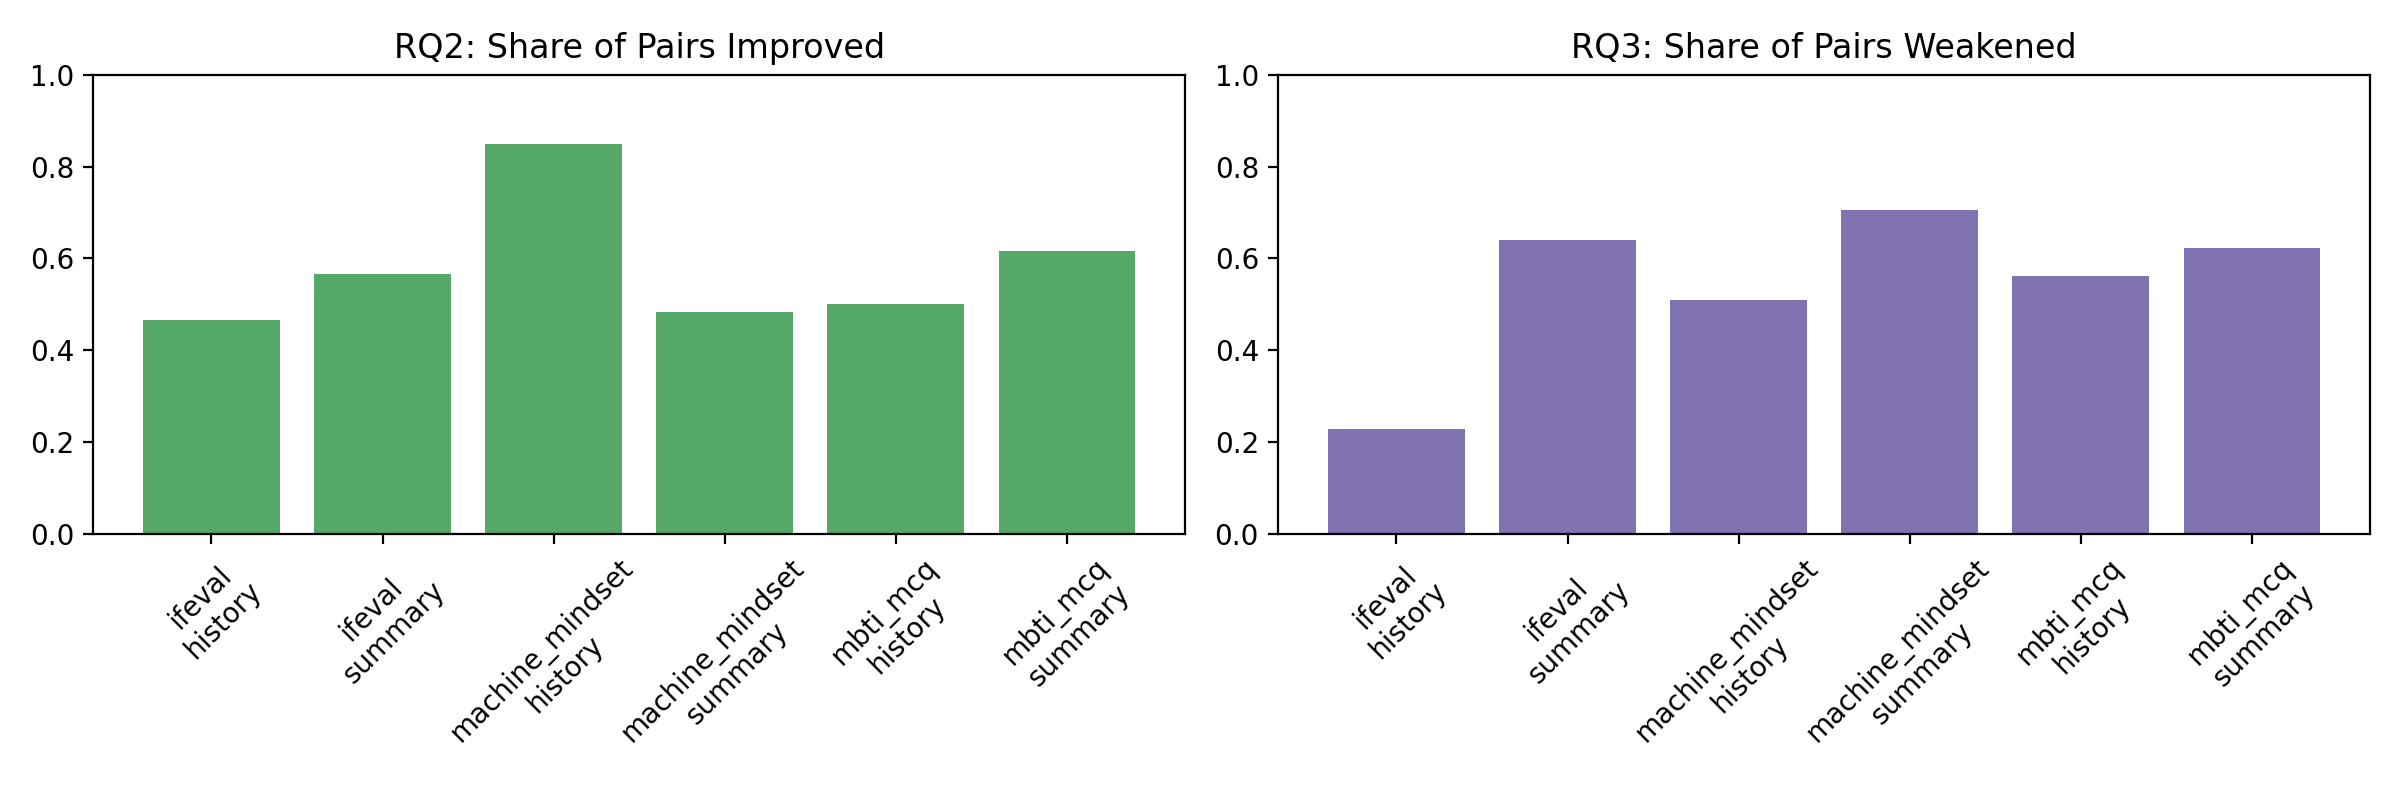
\includegraphics[width=0.92\linewidth]{final_report_assets/rq2_rq3_overview.png}
\caption{Stable-control-filtered full-run overview for the completed RQ2 and RQ3 pools. RQ2 still favors summary MBTI, while RQ3 shows weakening in both tracks and no summary immunity.}
\label{fig:rq2-rq3}
\end{figure}

\subsection{Systematic Failure Mode: Matched-Control Drift}

A key diagnostic result is that some failures arise even in the matched $B \rightarrow B$ control.
This means not every observed switch shortfall can be blamed on residual influence from persona $A$.

The strongest example is target ENTJ.
In our manual audit of matched-control MBTI profiles, RQ1 contains 11 drift pairs where the target is ENTJ but both matched controls land on ESTJ.
In the completed RQ2 run pool, six pair-tracks are removed for exactly this reason, and strong final updates do not eliminate the ENTJ-to-ESTJ boundary instability.
RQ3 adds another failure mode: for ISTP targets, several reinforced history controls drift toward ISTJ while the corresponding simple controls remain on ISTP.

These control drifts matter substantively.
They show that the model has local personality boundaries where even same-target controls are unstable.
Therefore, our matched-control design is not just useful; it is necessary.
Without it, one could incorrectly attribute all deviations from target persona $B$ to failed switching, when some are actually failures of the control itself.

\section{Analysis and Discussion}

The evidence supports a coherent causal story.
Earlier persona conditioning does persist into later behavior, but whether that persistence survives an explicit switch depends strongly on how earlier context is represented.
Raw history preserves too much low-level anchoring, including wording patterns and persona-consistent answer trajectories.
Compressed summary keeps the high-level narrative of the earlier interaction while discarding much of the token-level inertia that would otherwise compete with the final persona instruction.

This interpretation explains all three research questions together.
RQ1 shows that summary dramatically outperforms history.
RQ2 shows that stronger final instructions can improve switching, but the gains are conditional on the task and on the metric being used: MBTI still favors summary, while Machine Mindset shows larger directional improvement under history.
RQ3 shows that making the early context deeper increases carryover even after stable-control filtering, and the resulting degradation is not confined to raw history because summary is also vulnerable once reinforced warmup is strong enough.

The asymmetry analysis also matters.
Switching is not simply a function of distance between personas.
Some unordered pairs are directionally asymmetric, which implies that the source persona matters, not just the target persona.
In practical terms, this means multi-stage agents cannot assume that ``undoing'' a previous role is equally easy in both directions.

Finally, the dimension-level analysis suggests that persona control is not monolithic.
Thinking-feeling and extroversion-introversion are the hardest to erase under history, while judging-perceiving remains the hardest to rewrite fully even after summary compression.
This kind of axis-specific pattern would be invisible in a single scalar success rate.

\section{Limitations and Risks}

\begin{itemize}[leftmargin=*]
    \item \textbf{Single-model scope.} All validated results in this report come from Gemini-2.5-Flash-Lite. The carryover profile may differ for other models.
    \item \textbf{Executed-pool versus original downstream design.} The validated downstream analyses use the complete executed pools currently present in the workspace, which contain 66 RQ2 pairs and 66 RQ3 pairs after a 30+30 tranche and a 36+36 supplement. The report therefore prioritizes complete executed evidence over a strict reconstruction of the originally intended 60+60 design.
    \item \textbf{Task-specific interpretability.} MBTI is the cleanest direct probe, while Machine Mindset and IFEval mix persona effects with broader semantic and stylistic variation.
    \item \textbf{Boundary instability.} Some matched controls drift on their own, especially around ENTJ and ISTP, which limits how cleanly any single pair can be interpreted.
    \item \textbf{No formal significance testing.} Our analysis is paired and stratified, but it remains effect-size-focused rather than based on confidence intervals or permutation tests.
\end{itemize}

\section{Conclusion}

This project shows that persona carryover is a real and measurable source of behavioral variability in LLMs.
The strongest finding is simple: \emph{how} earlier context is retained matters more than merely strengthening the final instruction.
Across the completed runs, summary-based retention consistently produces cleaner switches than raw history.

The downstream interventions reinforce this conclusion.
RQ2 shows that stronger final instructions can partially repair switching, but the gains are selective and do not remove the constraints imposed by retained pre-switch context.
RQ3 shows that deeper early conditioning amplifies carryover, and the stable-control-filtered results indicate that even summary retention is not immune once the warmup signal is reinforced enough.
Taken together, these results suggest a practical recommendation: if an application needs reliable post-switch behavior, context compression is a stronger and more dependable control lever than prompt intensification alone.

\section*{Reproducibility Statement}

\begin{itemize}[leftmargin=*]
    \item Code repository: \texttt{persona-switch-carryover}
    \item Main experimental entry point: \texttt{python -m src.main}
    \item Main batch runners: \texttt{scripts/run\_rq2\_rq3\_selected\_60\_batch.py} and associated analysis scripts in \texttt{scripts/analysis/}
    \item Model: \texttt{gemini-2.5-flash-lite}
    \item Prompt families: MBTI persona prompts, warmup prompts, summary prompts, and task prompts stored in the repository
    \item Data used in validated analyses: MBTI questions (93), Machine Mindset sample (30), IFEval sample (30)
    \item Aggregated result files used in this report: \texttt{outputs/tables/rq1\_twoway240\_full\_run\_*}, \texttt{outputs/tables/rq2\_selected66\_stable\_control\_full\_run\_*}, and \texttt{outputs/tables/rq3\_selected66\_stable\_control\_full\_run\_*}
\end{itemize}

\begin{thebibliography}{9}

\bibitem{chen2023behavior}
Lingjiao Chen, Matei Zaharia, and James Zou.
\newblock How Is ChatGPT's Behavior Changing over Time?
\newblock 2023.

\bibitem{persona2024quantifying}
Anonymous.
\newblock Quantifying the Persona Effect in LLM Simulations.
\newblock 2024.

\bibitem{greedy2024nondeterminism}
Anonymous.
\newblock The Good, The Bad, and The Greedy: Evaluation of LLMs Should Not Ignore Non-Determinism.
\newblock 2024.

\bibitem{helpful2024personas}
Anonymous.
\newblock When ``A Helpful Assistant'' Is Not Really Helpful: Personas in System Prompts Do Not Improve Performances of Large Language Models.
\newblock 2024.

\bibitem{deterministic2025nondeterminism}
Anonymous.
\newblock Non-Determinism of ``Deterministic'' LLM Settings.
\newblock 2025.

\bibitem{control2025illusion}
Anonymous.
\newblock Control Illusion: The Failure of Instruction Hierarchies in Large Language Models.
\newblock 2025.

\end{thebibliography}

\end{document}
